% !TEX root = ../../../main.tex

\toggletrue{image}
\toggletrue{imagehover}
\chapterimage{python_environment}
\chapterimagetitle{\uppercase{Python Environment}}
\chapterimageurl{https://xkcd.com/1987/}
\chapterimagehover{The Python environmental protection agency wants to seal it in a cement chamber, with pictorial messages to future civilizations warning them about the danger of using sudo to install random Python packages.}

\chapter{Parameter}
\label{ch:parameter}

\vspace{-0.25cm}

Wir kennen bereits Funktionen, die beim Funktionsaufruf ein Argument benötigen.

\begin{example}
Die Funktion \lstinline[language={python3}]{forward} wird mit einem Argument aufgerufen. Das Argument ist ein Integer. Bei \lstinline[language={python3}]{forward(100)} ist das Argument der Integer \lstinline[language={python3}]{100}.
\end{example}

Damit wir beim Funktionsaufruf ein Argument übergeben können, müssen wir bei der Funktionsdefinition einen \textbf{Parameter} definieren. Dies schauen wir uns nun an. Die Lernziele lauten:\\

\lernziel{\autoref{ch:parameter}, \nameref{ch:parameter}}{
\begin{minipage}{\linewidth}
$\square$ \hspace{0.1cm} Sie erklären das Prinzip der Parameter anhand eines Beispiels.\\
$\square$ \hspace{0.1cm} Sie erstellen Ihre eigene Funktion mit einem oder mehreren Parametern.\\
$\square$ \hspace{0.1cm} Sie rufen eine eigene Funktion mit einem oder mehreren Parametern auf.\\
$\square$ \hspace{0.1cm} Sie verwenden Funktionen mit Parametern, um Code bei einem Mausereignis auszuführen.
\end{minipage}
}

\vspace{-0.5cm}

\section{Vier Quadrate \Ninja[][white]}

Wir können mit dem Programm aus \autoref{lst-vier-quadrate} die Figur aus \autoref{figure-vier-quadrate} zeichnen.

\vspace{-0.25cm}

\begin{figure}[H]
\centering
\begin{minipage}[c][4cm]{0.5\linewidth}
\centering
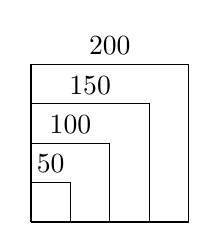
\begin{tikzpicture}
	\draw (0,0) -- ++(0.5cm, 0) -- ++(0, 0.5cm) to node [sloped, above] {$50$} ++(-0.5cm, 0) -- ++(0, -0.5cm);
	\draw (0,0) -- ++(1cm, 0) -- ++(0, 1cm) to node [sloped, above] {$100$}  ++(-1cm, 0) -- ++(0, -1cm);
	\draw (0,0) -- ++(1.5cm, 0) -- ++(0, 1.5cm) to node [sloped, above] {$150$} ++(-1.5cm, 0) -- ++(0, -1.5cm);
	\draw (0,0) -- ++(2cm, 0) -- ++(0, 2cm) to node [sloped, above] {$200$} ++(-2cm, 0) -- ++(0, -2cm);
\end{tikzpicture}
\caption{Das Programm aus \autoref{lst-vier-quadrate} zeichnet vier unterschiedlich grosse Quadrate.}
\label{figure-vier-quadrate}
\begin{justify}
Wir können die Seitenlänge der Quadrate auf einfache Weise anpassen, indem wir bei der Funktionsdefinition einen Parameter notieren (Zeile 4). Ein Parameter ist eine spezielle Variable. Beim Funktionsaufruf können wir dann ein Argument übergeben (Zeile 10, Zeile 11 und Zeile 12).
\end{justify}
\end{minipage}
\hfill
\begin{minipage}[c]{0.45\linewidth}
\centering
\begin{lstlisting}[language={python3}, caption={\graybgtexttt{vier\_quadrate.py}}, label={lst-vier-quadrate}]
import turtle as t


def quadrat(seitenlaenge):
	for _ in range(4):
		t.fd(seitenlaenge)
		t.lt(90)


def quadrate():
	quadrat(50)
	quadrat(100)
	quadrat(150)
	quadrat(200)


quadrate()
t.done()

\end{lstlisting}
\end{minipage}
\end{figure}

\section{Parameter definieren}

Wir können in der Funktionsdefinition \textbf{zwischen} den Klammern Parameter definieren.

\begin{definition}[Parameter]
Ein Parameter ist eine spezielle \textbf{Variable} der Funktion. Die Variable steht nur innerhalb der Funktionsdefinition zur Verfügung. Ein Parameter ist also eine \textbf{lokale Variable}. Wir definieren einen oder mehrere Parameter bei der Funktionsdefinition \textbf{zwischen} den runden Klammern. \textbf{Mehrere Parameter} werden durch \textbf{Kommata} getrennt.
\end{definition}

\begin{example}
In \autoref{lst-vier-quadrate} wird in Zeile vier bei der Funktionsdefinition ein Parameter verwendet. Der Parametername lautet \lstinline[language={python3}]{seitenlaenge}.
\end{example}

\begin{important}
Beim Funktionsaufruf muss für \textbf{jeden} Parameter ein \textbf{Argument} vorhanden sein. Man muss jedem Parameter einen Wert übergeben.
\end{important}

\subsection{Wie wählen wir Parameternamen?}

Im Rahmen der üblichen Regeln sind wir bei der Wahl des Parameternamens grundsätzlich frei. Es wird jedoch empfohlen, den Parameternamen so zu wählen, dass allein aus dem Parameternamen ersichtlich ist, wofür der Parameter verwendet wird.

\vspace{-0.25cm}

\cleancoderegel{\autoref{ch:parameter}, \nameref{ch:parameter}}{
\begin{cleancode}[Sinnvolle Parameternamen]
Wir wählen die \textbf{Parameternamen} so, dass wir sofort verstehen, wofür der Parameter verwendet wird.
\end{cleancode}
}

\vspace{-0.25cm}

\begin{important}
Hat eine Funktionsdefinition mehrere Parameter, so muss jeder Parametername eindeutig sein.
\end{important}

\vspace{-0.5cm}

\cleancoderegel{\autoref{ch:parameter}, \nameref{ch:parameter}}{
\begin{cleancode}[Snake Case für Parameternamen]
Da ein Parameter eine lokale \textbf{Variable} darstellt, verwenden wir auch für \textbf{Parameternamen} die Snake Case-Notation.
\end{cleancode}
}

\vspace{-0.5cm}

\section{Variablen beim Funktionsaufruf}

Wir können beim Funktionsaufruf auch eine \textbf{Variable} verwenden. \autoref{lst-vier-quadrate-variante} zeigt, wie wir die Figur aus \autoref{figure-vier-quadrate} mit einer \lstinline{for}-Schleife zeichnen können.

\begin{lstlisting}[language={python3}, caption={Variable beim Funktionsaufruf (\graybgtexttt{vier\_quadrate\_variante.py}).}, label={lst-vier-quadrate-variante}]
import turtle as t


def quadrat(seitenlaenge):
	for _ in range(4):
		t.fd(seitenlaenge)
		t.lt(90)


def quadrate():
	a = 50
	for _ in range(4):
		quadrat(a)
		a = a + 50


quadrate()
t.done()

\end{lstlisting}

\section{Mehrere Parameter}

Wir können beliebig viele Parameter für eine Funktion definieren. 

\begin{important}
Beim Funktionsaufruf spielt die \textbf{Reihenfolge der Parameter} eine Rolle: Die Argumente müssen in der gleichen Reihenfolge wie die Parameter angegeben werden.
\end{important}

\begin{example}
\autoref{lst-vier-bunte-quadrate} zeigt ein Beispiel mit zwei Parametern. Der erste Parameter der Funktion \lstinline[language={python3}]{quadrat} bestimmt die Seitenlänge des Quadrats. Der zweite Parameter bestimmt die Linienfarbe.
 
\begin{lstlisting}[language={python3}, caption={Funktion mit zwei Parametern (\graybgtexttt{vier\_bunte\_quadrate.py}).}, label={lst-vier-bunte-quadrate}]
import turtle as t
import random as r


def quadrat(seitenlänge, farbe):
	t.pencolor(farbe)
	for _ in range(4):
		t.fd(seitenlänge)
		t.lt(90)


def quadrate():
	for _ in range(4):
		farbe = r.choice(["red", "green", "blue"])
		quadrat(50, farbe)
		t.pu()
		t.fd(125)
		t.pd()


quadrate()
t.done()

\end{lstlisting}
\end{example}

Es dürfen auch mehrere Funktionen definiert werden, welche mehrere Parameter besitzen.

\cleancoderegel{\autoref{ch:parameter}, \nameref{ch:parameter}}{
\begin{cleancode}[Leerzeichen 7]
    Mehrere \textbf{Parameter} werden durch ein \textbf{Komma} getrennt. \textbf{Nach} einem Komma notieren wir ein \textbf{Leerzeichen}.
\end{cleancode}
}

\section{Mausereignisse verarbeiten}

Mit der Funktion \lstinline[language={python3}]{onscreenclick} registrieren wir eine \textbf{Funktion}, die beim Klicken der Maustaste einmalig ausgeführt wird. Wird die Maustaste zweimal hintereinander gedrückt, wird die Funktion zweimal hintereinander ausgeführt. Die Funktion \lstinline[language={python3}]{onscreenclick} benötigt nur ein Argument beim Funktionsaufruf. Es muss der \textbf{Funktionsname} übergeben werden, damit beim Mausklick die richtige Funktion aufgerufen wird.

\begin{important}
Das Argument ist \textbf{nur der Funktionsname} - keine runden Klammern!
\end{important}

Damit die Mausereignisse verarbeitet werden, müssen wir \textbf{nach der Registrierung einmal} die \lstinline[language={python3}]{listen}-Funktion aufrufen. Bei der \textbf{Funktionsdefinition} zur Verarbeitung des Mausklicks müssen \textbf{zwei Parameter} notiert werden. Der erste Parameter speichert die \textbf{x-Koordinate} und der zweite Parameter die \textbf{y-Koordinate} des Mausklicks. Diese können wir dann in der Funktion verwenden.

\begin{example}
\autoref{lst-quadrate-funktion-maus} zeigt ein Beispiel, wie wir für jeden Mausklick ein Quadrat zeichnen können. Die Parameter \lstinline[language={python3}]{x} und \lstinline[language={python3}]{y} speichern die Koordinaten des Mausklicks. Wir bewegen dann die Turtle zu dieser Position und zeichnen dort das Quadrat mit der Seitenlänge $50$.

\begin{lstlisting}[language={python3}, caption={Bei jedem Mausklick wird die Funktion einmal ausgeführt. (\graybgtexttt{quadrate.py}).}, label={lst-quadrate-funktion-maus}]
import turtle as t


def quadrat_<@\color{black}{50}@>(x, y):
	t.pu()
	t.goto(x, y)
	t.pd()
	for _ in range(4):
		t.fd(50)
		t.lt(90)


t.onscreenclick(quadrat_<@\color{black}{50}@>)
t.listen()
t.done()
\end{lstlisting}
\end{example}

\vfill

\begin{figure}[H]
\centering
\uppercase{Frankenstein Captcha} \\
\includegraphics[scale=0.75]{frankenstein_captcha_2x}
\caption*{The distinction between a ship and a boat is a line drawn in water.\footnotemark}
\end{figure}

\footnotetext{\url{https://xkcd.com/2604/}}